\section{Motivation}
Technologies have revolutionised the manufacturing industry ever since the Industrial revolution in the 19th century. Robots have increased productivity by replacing humans for arduous and repetitive manual tasks. Autonomous robots have been able to increase efficiency, lower costs, and relieve humans from operationally dangerous tasks. There has been a noticeable increase in industrial robot order requests, as well as capital investments into the field. Although robots can be superior in automating human tasks,  there remain many tasks that cannot be completely taken over and that still need human intervention, such as high-precision tasks. Traditional robot programming requires robotics and programming experts. This is a bottleneck for industries as they cannot change robot functions easily.
To overcome this difficulty, recent research has been focusing on robot programming for end-users.


\subsection{Cobotics}\label{subsec:Cobotics}
Collaborative robots, or ``cobots", have been introduced by Peshkin and Colgate in 1999 \cite{colgate1999cobots}. With the goal to automate repetitive and manual tasks, cobotics allows a close collaboration between humans and robots. Cobots contribute to productivity gains as they are designed to respond to actions of the human operator. They enable humans to perform tasks, which they cannot perform on their own, due to physical constraints such as the manipulation of heavy parts. Furthermore, they reduce risks of work-related accidents, including health hazards such as exposure to dangerous environments (e.g. chemical acids, excessive temperatures or noise), as well as sleeping disorders caused by rotating work shifts. 

Cobotic systems have been adapted in several industries from the food-processing industry \cite{Food}, to aeronautics \cite{Airbus} to the health industry \cite{Ebola}. Despite the uptake of the robotics technology, there exist strong barriers, which prevent their widespread adoption. Companies, which resist the use of robots in their daily routines, perceive no actual need for them and consider the investment cost ineffective, due to their high initial costs. Another factor is the lack of trained personnel, who have the required skills to fully operate and exploit the robots. The use of cobots opens up a market for new high-skilled jobs, while replacing those of low-skilled human workers.


\subsection{Robot Programming by Demonstration}
Classical robot programming processes in the industry have task-specific definitions, which are generally robot-dependent, and require programming expertise. Figure \ref{fig:Classical robot programming process} shows the classical robot programming process. After the initial task definition, an optimal sequence of the workcell operations is defined. Once the process has been validated, the robot is programmed offline in its native language, before it is pushed into production for regular execution. The programmed robot can only be used for this specific task, in this particular working environment. If the task definition needs to be altered, the programming expert needs to repeat the entire programming process. Therefore, classical robot programming processes are time consuming and cost intensive.

  \begin{figure}[ht]
    \centering
    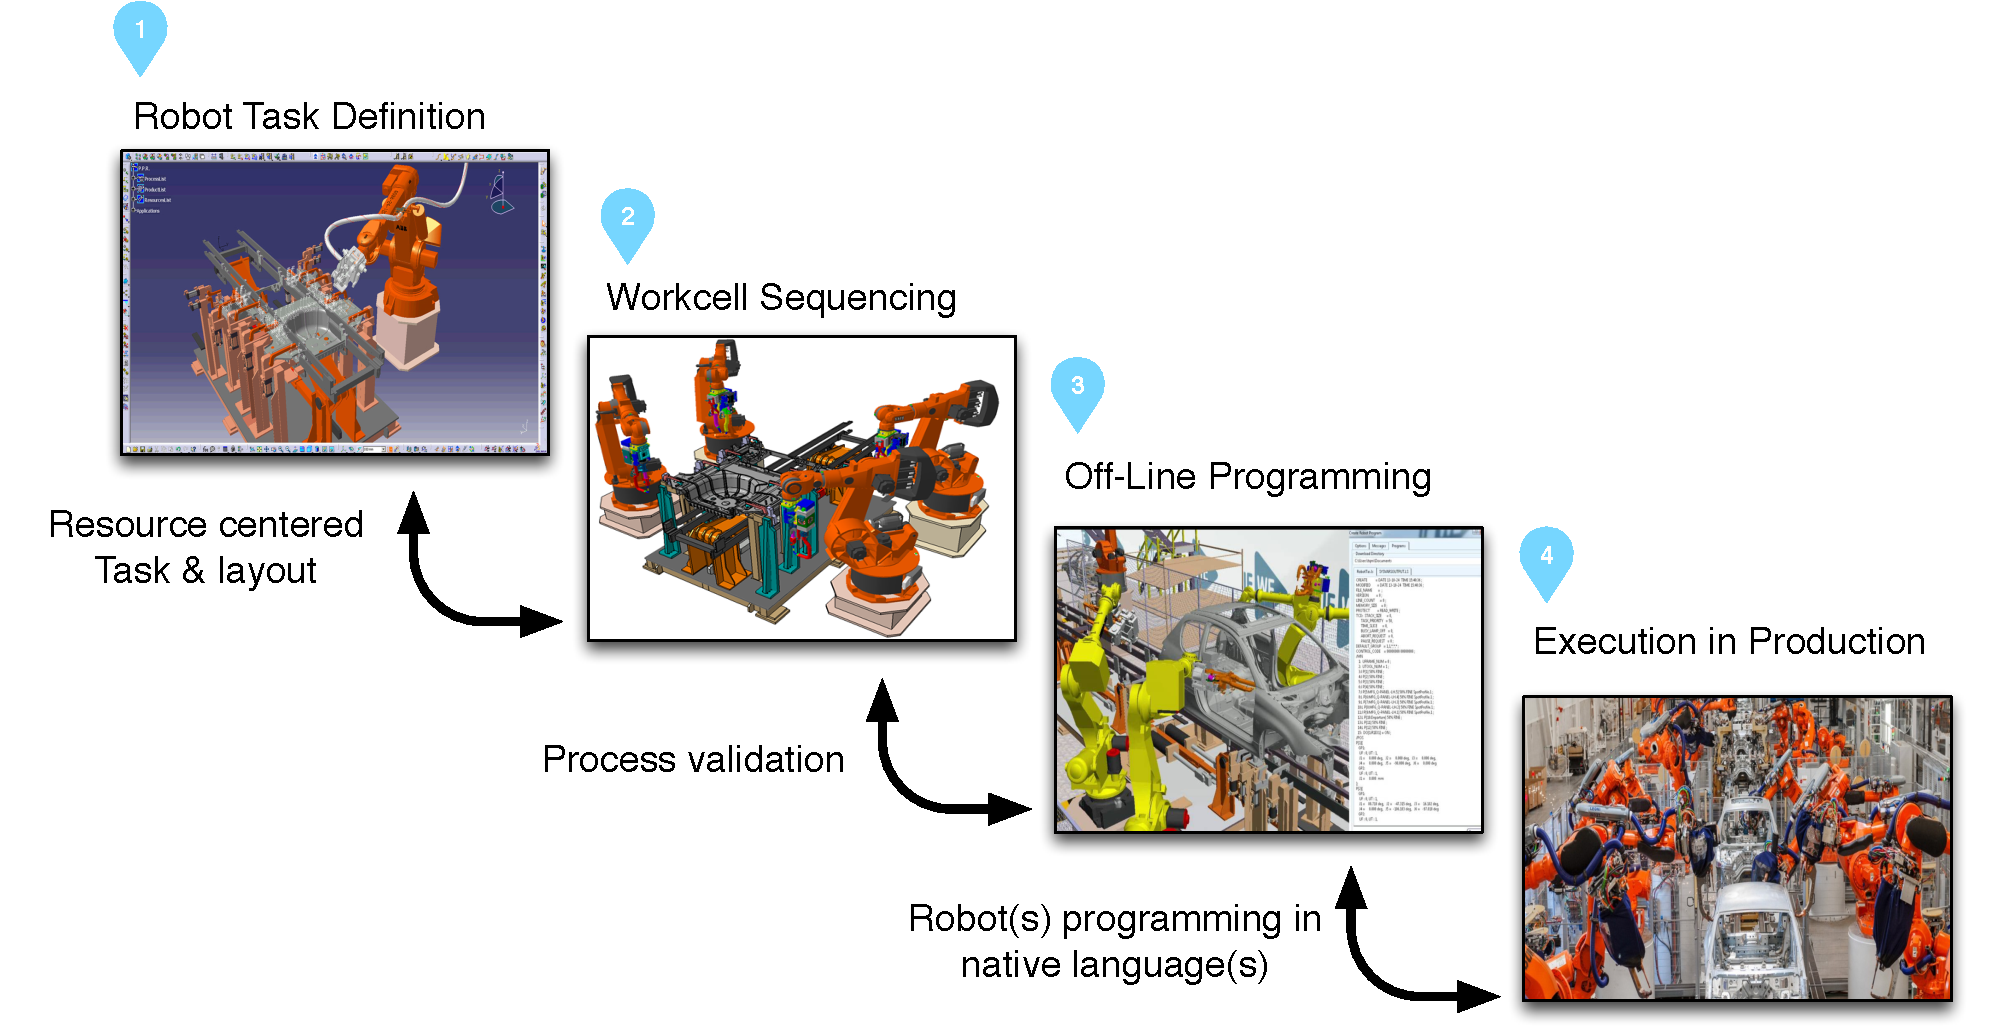
\includegraphics[scale=0.4]{figures/manual-programming}
    \caption{Classical robot programming process}
    \label{fig:Classical robot programming process}
  \end{figure}

Robot Programming by Demonstration (PbD), also referred to as \textit{Robot Learning from Demonstration}, is a technique for teaching a robot new behaviours simply by demonstrating a task, instead of explicitly programming them through machine commands \cite{ghallab2004automated}.
PbD has become a central topic in research areas, with the aim to move from purely pre-programmed robots to flexible user-based interfaces for training robots \cite{billard2008robot}. Influenced by natural learning paradigms in humans and other animals, the ultimate goal is to develop an intuitive method for programming that can be used by untrained, na\"{\i}ve users \cite{suay2012practical}. The aim is to continually refine the performance of the robot by repetitive demonstrations. 


Figure \ref{fig:Principle Overview} shows the life-cycle for teaching a robot by demonstration. 
The teacher demonstrates the desired behaviour to the robot. The robot uses its different sensors for a multi-modal perception of the demonstration and extracts the relevant information, to create a model of the skill. The new skill is evaluated via execution in a new context, under the supervision of the teacher. The teacher can refine the learned skill by presenting demonstrations of the same skill under different conditions. The robot then generalises over the different demonstrations by extracting essential components that remained unchanged across the various demonstrations. This incremental learning process allows the robot to perform the learned task straight away, while being monitored by the teacher, and therefore allows the robot to learn a task from as few demonstrations as possible \cite{billard2008robot}. 

  \begin{figure}[h]
    \centering
    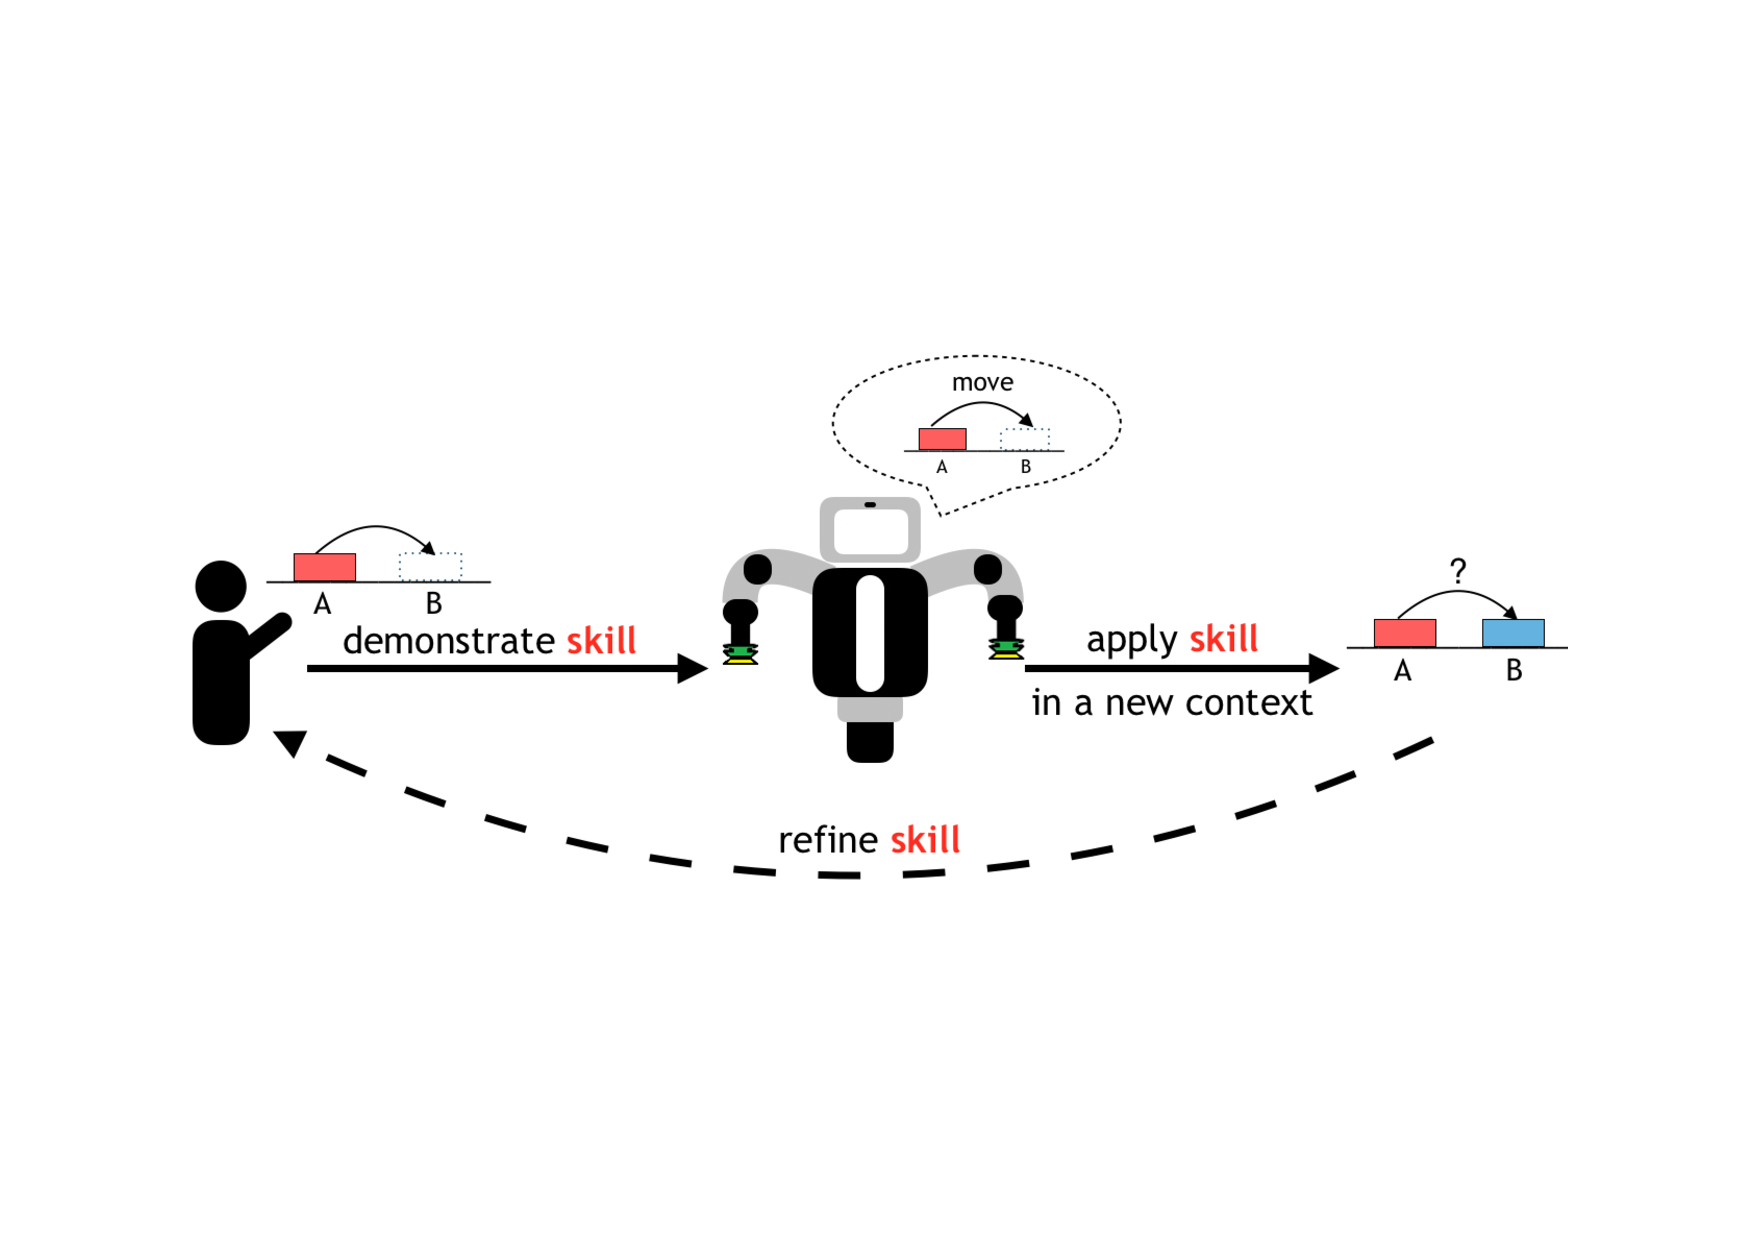
\includegraphics[scale=0.7]{figures/PbD-Overview}
    \caption{PbD Overview}
    \label{fig:Principle Overview}
  \end{figure}

%Besides the advantage of being able to teach the robot tasks without the need to write code, PbD provides a powerful tool to improve learning abilities by reducing the search space of possible solutions. 

\subsection{Challenges in Robot PbD}
Despite there being many PbD algorithms proposed in research literature (\cite{argall2009survey}, \cite{billing2010formalism}), there still remain several research challenges that address the suboptimality of demonstrations (\cite{chen2003programing}, \cite{kaiser1995obtaining}) or the lack of comparative user studies (\cite{suay2012practical}).
Learning object manipulation tasks is considered a hard problem, as the robot has limited world knowledge due to restricted sensor availability \cite{ekvall2008robot}. 
Furthermore, existing PbD implementations are not goal-oriented. The robot is taught a task execution, which achieves a goal, but it cannot deduce a task execution from a given goal. Current PbD approaches only teach the robot the action of manipulating an object, but do not explicitly associate a semantic meaning to it, other than assigning it a  name. In this project, we will concentrate on teaching the robot not only an object manipulation task, but also its semantic meaning, so that it understands the relevant application context.

For example, the robot is taught to pick up an object from an initial position and place it on a goal position. Conditions for executing this action (e.g. grab an object only if the gripper is free) are generally neglected during the demonstration. %These conditions are usually programmed into the robot. % or the robot is faced with a perfect scenario \cite{x}. %find example in paper 
If the teacher demonstrates a pick-up action to the robot, there is no mention of communicating the conditions for when it can execute the action. 
%Implementations, which take a user interface to select task execution plans \cite{guerin2015framework}.

%One of the main challenges in PbD is to teach the robot a generic task that can be applied to generic scenarios especially when the task setting has been changed. A robot that learns how to arrange items on a desk may have to plan the order of handling differently sized objects in another way than originally demonstrated by the teacher. Thus, it does not suffice for the robot to replicate the demonstrated movement, but it needs to understand and interpret the teacher's intention so that it can apply the action to multiple scenarios. Learning object manipulation tasks is considered a hard problem due to the robot's limited world knowledge and constraints of available sensors \cite{ekvall2008robot}.

%suboptimality of demonstrations
%Another known PbD problem exists with regards to the type and quality of the demonstration which is dependent on the teacher's knowledge of the robot's system. Na\"{\i}ve teachers may have greater assumptions on the robot's intelligence and take less care in executing demonstrations as compared to roboticists, who understand the effects of noisy demonstrations \cite{suay2012practical}. \cite{chen2003programing} and \cite{kaiser1995obtaining} recognised different sources for sub-optimality in demonstration such as the user demonstrating unnecessary or incorrect actions due the lack of knowledge about the task.

%lack of comparisons between algorithms
%Despite there being many PbD algorithms proposed in research literature (\cite{argall2009survey}, \cite{billing2010formalism}), there remains a lack in comparative user studies. Difficulties in comparing across applications arise from the use of different robotic platforms and demonstration techniques, which lead to different representations of demonstration data. \cite{suay2012practical} partly addresses this challenge by comparing three well-established algorithms and evaluating their performance in a common domain.

Consider the task of permutating two objects, which are red and blue and located at positions A and B respectively. Our goal is to permutate the two objects, such that red is located at B and blue at A (see Figure \ref{fig:Permutation}). The robot is only equipped with one arm and provided with three positions A, B and C. As humans, we naturally understand that we need to empty one of the two occupied goal positions (A or B), by making use of the empty space C. If the robot was only taught to move objects, but not the conditions for moving them (i.e. that the goal position needs to be vacant before placing an object), it will not be able to produce the same reasoning as us. As existing PbD implementations are not goal-oriented, the robot needs to be taught the precise action sequence for the permutation of two objects.

  \begin{figure}[h]
    \centering
    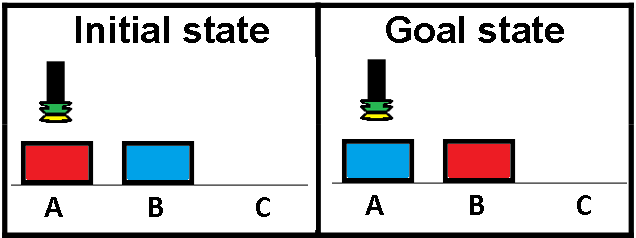
\includegraphics[scale=0.35]{figures/PbD-permutation}
    \caption{Initial state and goal state for the permutation of two objects}
    \label{fig:Permutation}
  \end{figure}
The act of placing an object from one position to another needs to be associated with the condition of having an empty goal position prior to action execution. In other words, we set a \textit{precondition} (\textit{``goal position is empty"}) on the state of the world, which needs to be fulfilled for this action to be executed. Similarly, we can set conditions for the state of the world \textit{after} the action execution, known as \textit{effects}, e.g. \textit{``object is at goal position"}. Thus, an \textit{action model} for the pick-and-place action consists of the following conditions:

\begin{table}[h]
\begin{center}
\begin{tabular}{l|l}
Preconditions & Effects\\ \hline
 & \\
The object X is at the initial position A. & The object X is at the goal position B.\\
The goal position B is empty. & The object X is not at the initial position A.
\end{tabular}
\end{center}
\label{tab:conditions}
%\caption{Preconditions an}
\end{table}

\noindent This representation, in terms of preconditions and effects, is used in Automated Planning techniques. It allows the robot to reason about its tasks by keeping track of the state of the world after each action execution. Using these action models, automated planners can generate an action sequence to achieve a goal. However, automated planners rely on a classical planning language called PDDL, which represents the conditions in first-order logic (see Figure \ref{fig:Pick-up action model}). %Action models, with conditions in first-order logic (see Figure \ref{fig:Pick-up action model}), are used to generate sequences of actions, known as \textit{plans}, to achieve a goal. 

  \begin{figure}[h]
    \centering
    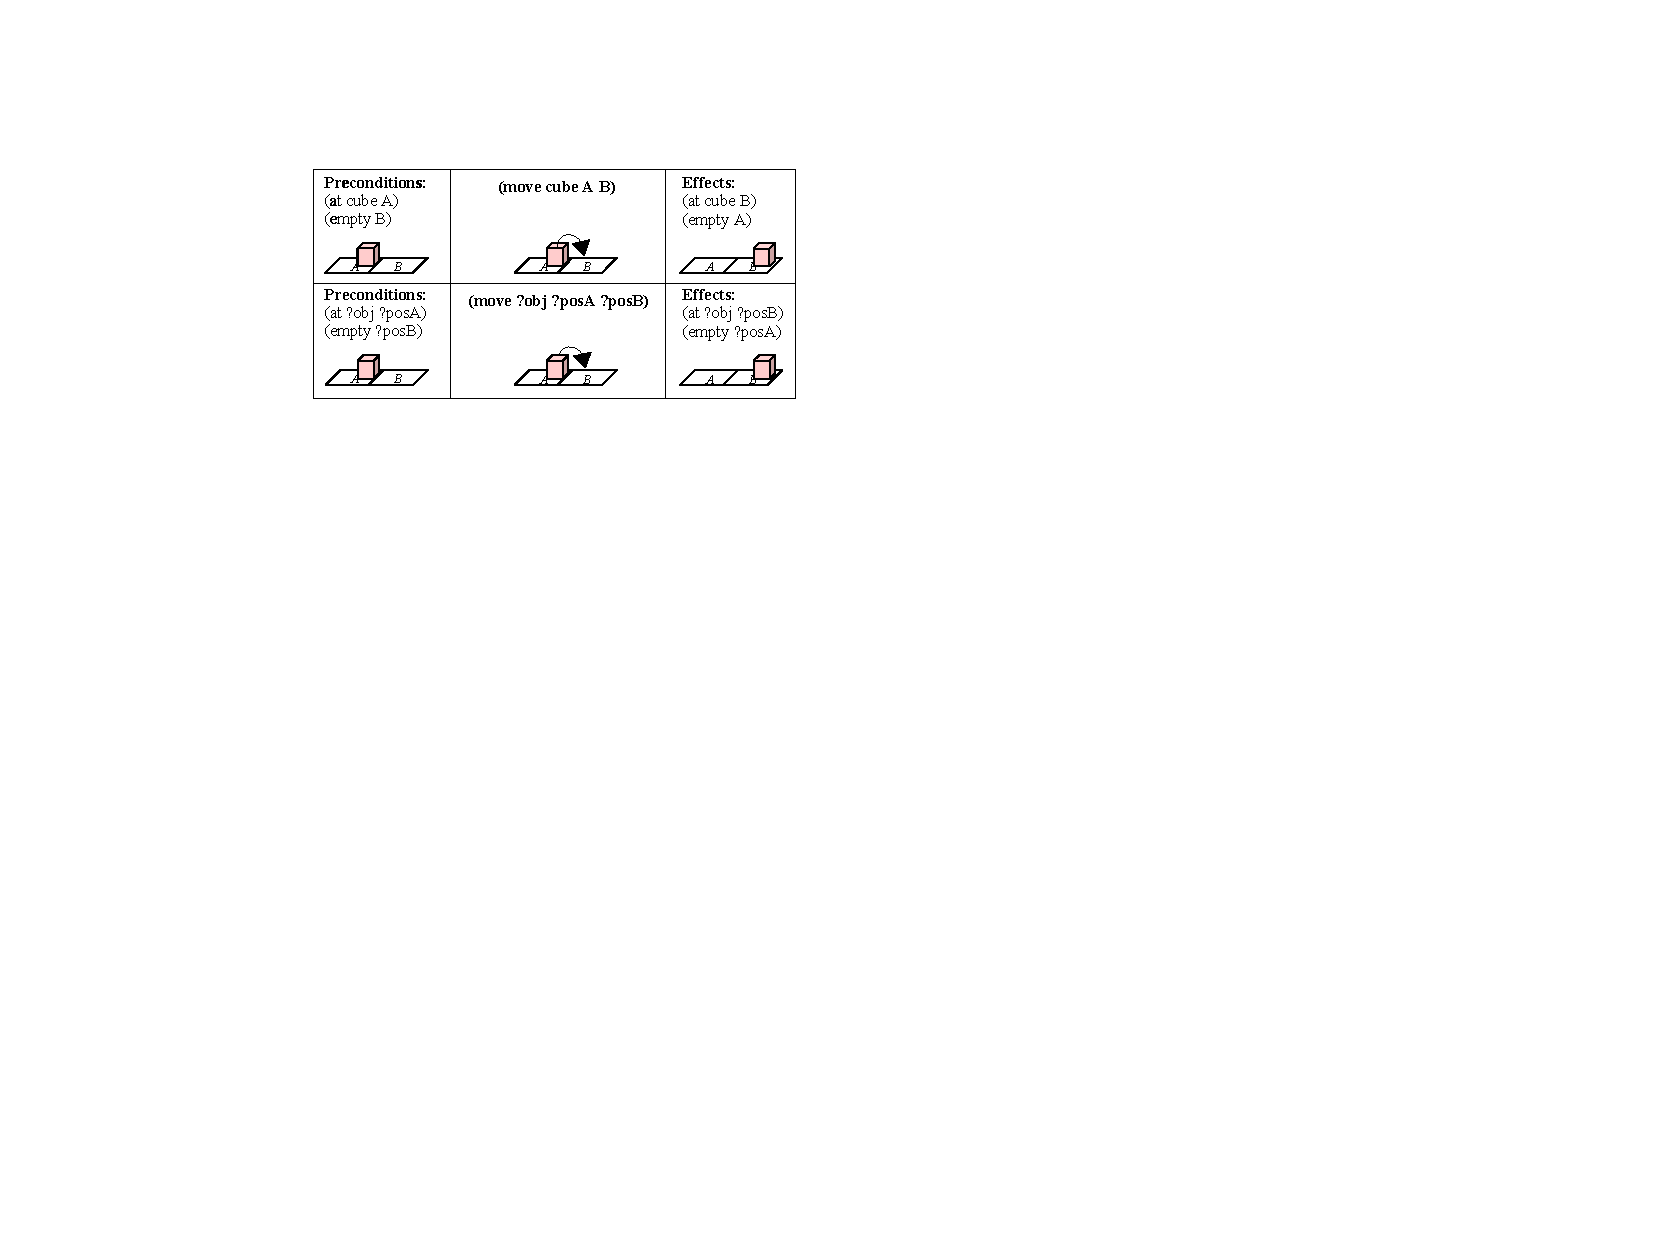
\includegraphics[scale=0.4]{figures/schema-logic}
    \caption{Action model representation in first-order logic}
    \label{fig:Pick-up action model}
  \end{figure}
Recall the example given earlier to permutate two objects (see Figure \ref{fig:Permutation}). Given an initial state (object red at position A, object blue at position B) and a goal state (object red at position B, object blue at position A), the planner can automatically generate an action sequence, which, if executed successfully, transitions from the initial state to the goal state: \texttt{move(blue,B), move(red,B), move(blue,A)} (see Figure \ref{fig:Automated Planner}).

  \begin{figure}[h]
    \centering
    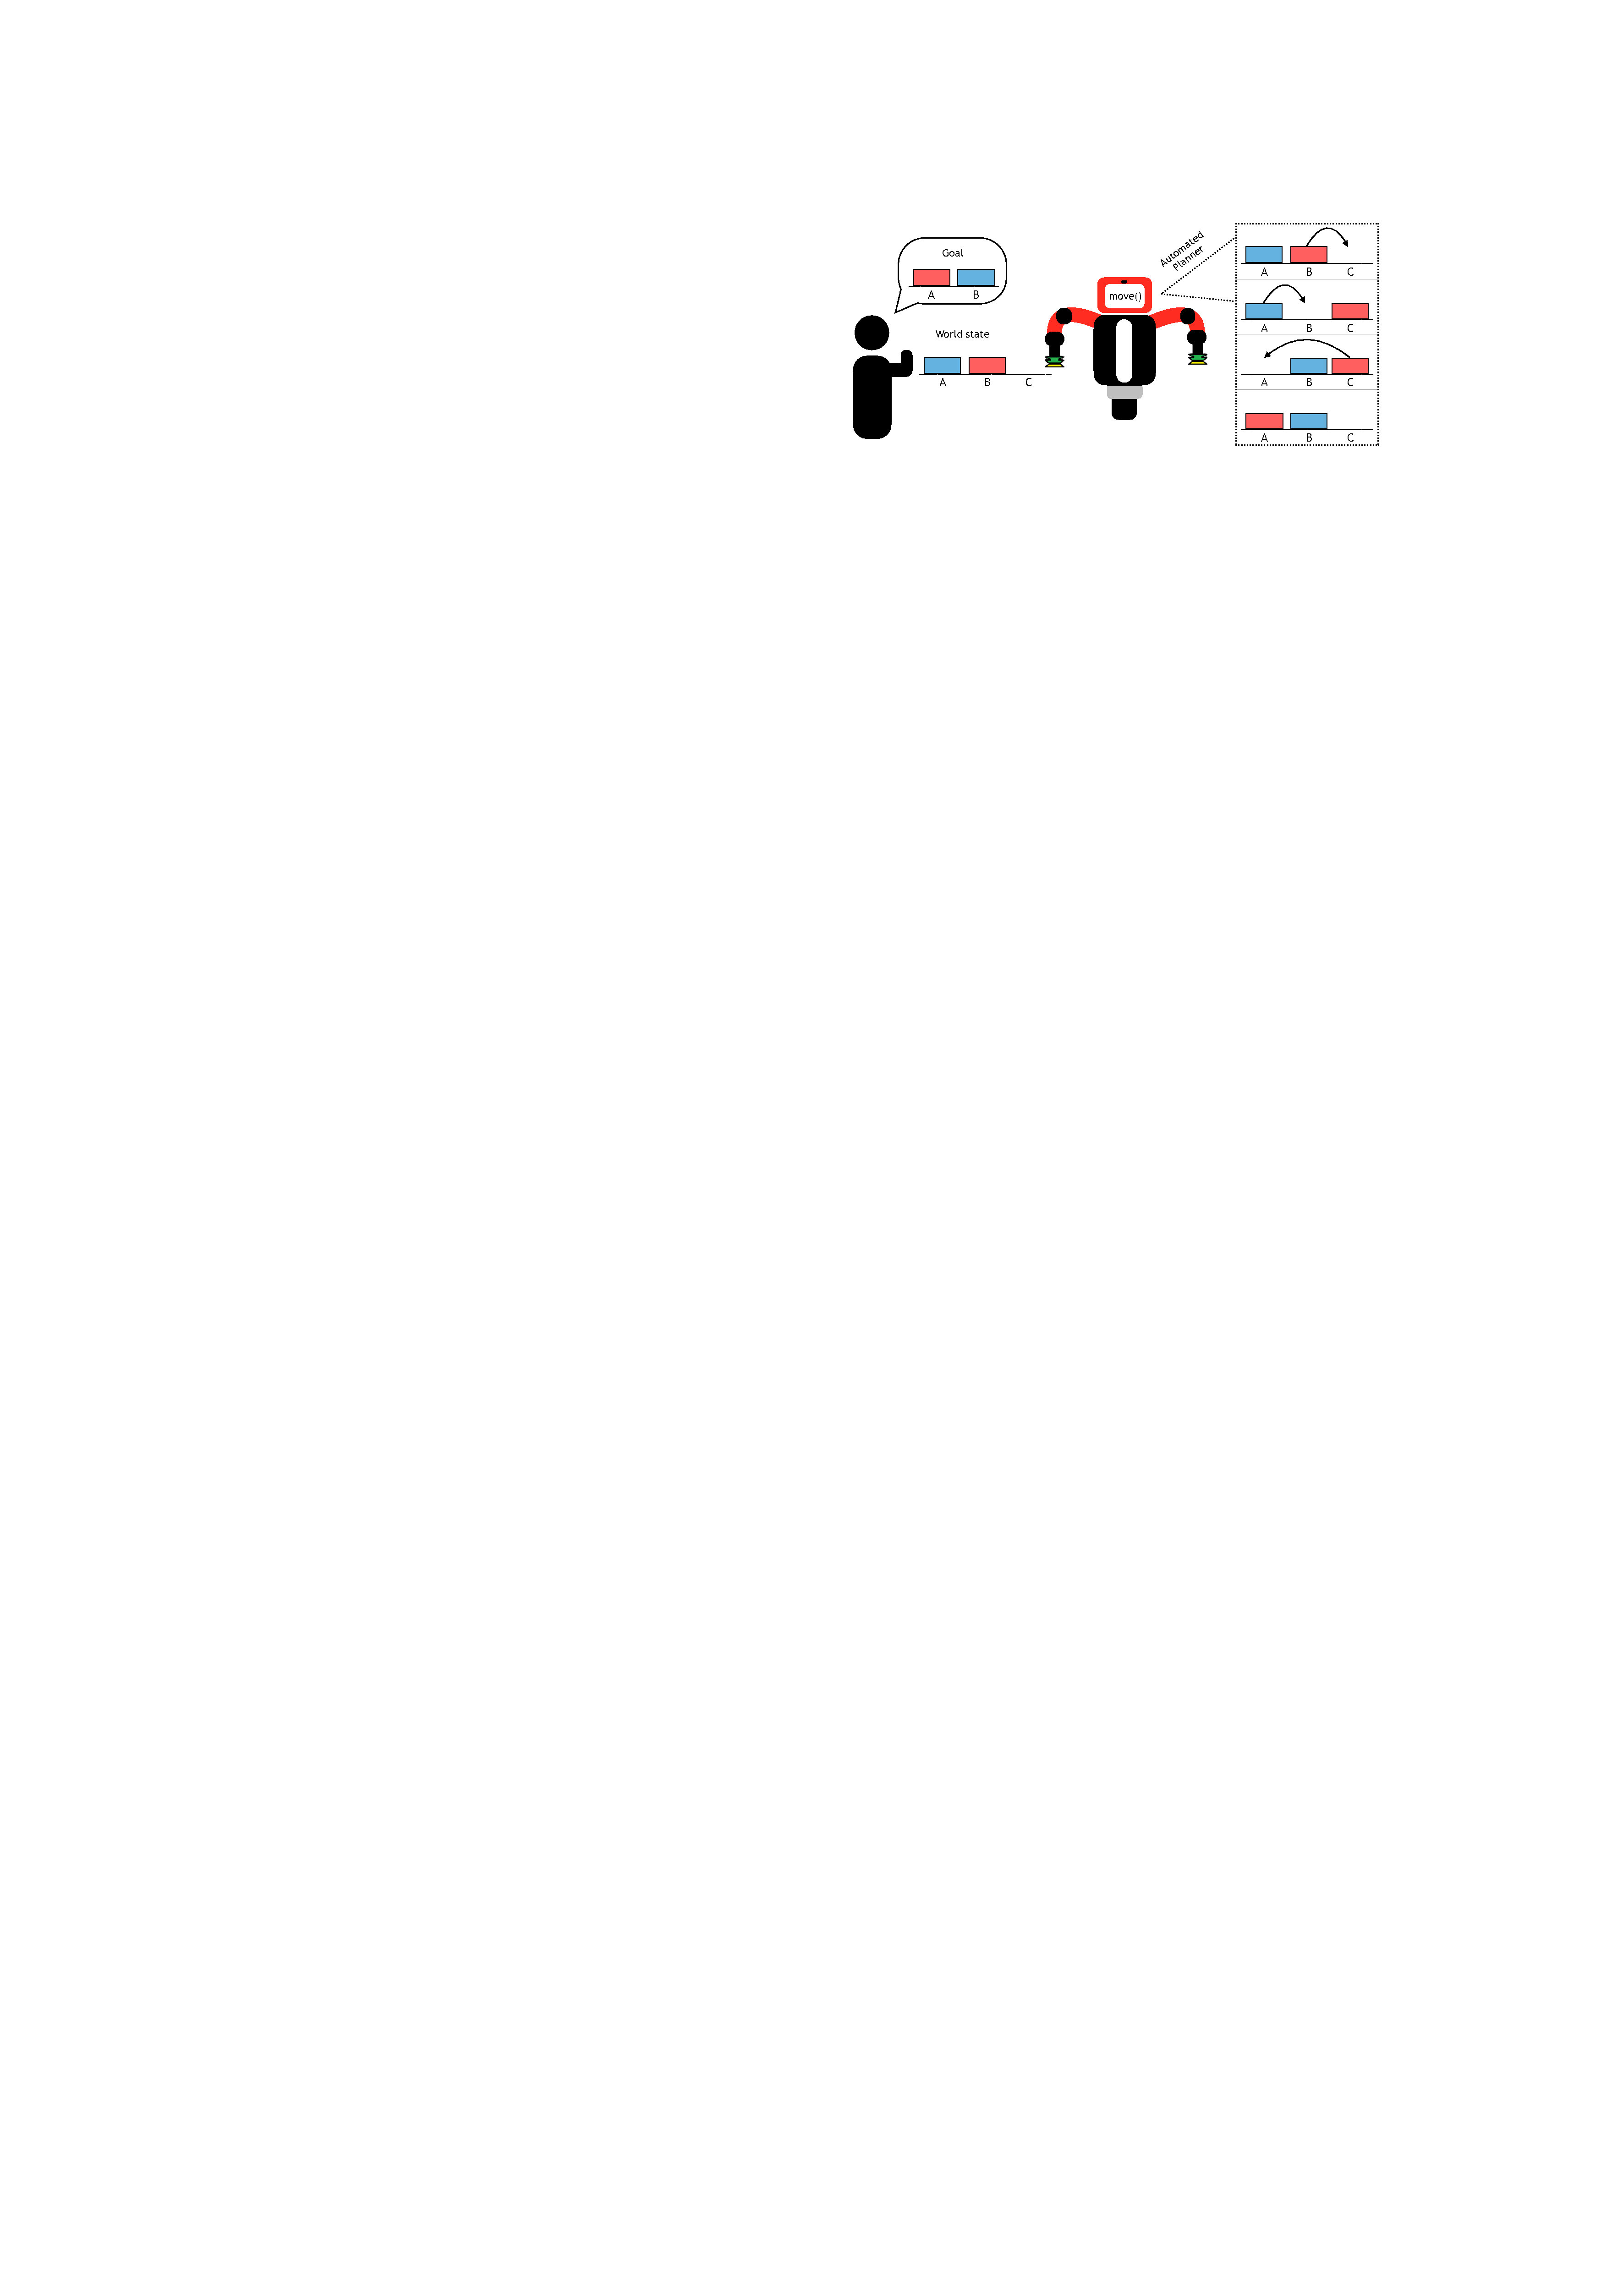
\includegraphics[scale=0.6]{figures/PbD-AutomatedPlanner}
    \caption{Action sequence automatically generated by an automated planner}
    \label{fig:Automated Planner}
  \end{figure}